% \externaldocument{2/chapter2.tex}
% \externaldocument{3/chapter3.tex}
\section{Biological Systems}
\label{sec:biosys}
The process of science is at its core nothing but a method to isolate phenomena to singular factors to attribute a cause to an effect. However, as we have seen, such isolation can be detrimental to the accuracy of the observation being gleaned. Thus, many if not all fields of science have long applied analytic tools developed alongside various branches of mathematics to ensure that while many factors are considered, their main observation is the most likely result of some initial cause. So too systems biology attempts to further quantize the realm of biology to more reflectively model natural systems in their native state, accounting for ever more variables in the process while maintaining confidence in the correlation of their experimental outcome.

\subsection{Stability}
\label{sec:stab}
As alluded to in \cref{sec:regwhatwhen}, natural systems have the ability to fluctuate in response to any number of internal and external stimuli, \eg up-regulating heat shock protein (HSP) in response to excess heat. In a similar manner to new growth media spurring rapid growth in bacterial cultures only to plateau and eventually die off if left alone, this HSP up-regulation is a momentary disturbance from a previous balance, a state of intermediate HSP levels, stable enough to call for more or less as the situation should demand. In characterizing HSP level in response to excess heat, one might expect a large increase in mRNA levels while heat persists. Similarly, after targeted gene knockdown, mRNA levels of said gene gradually decrease as indirect gene partners feel the effects of their partners decreased presence. A state of zero net change is only reached after the system has adapted to this new, decreased but not characteristically altered state as time is allowed to run (\cref{fig:SS}).

\begin{figure}[H]
\centering
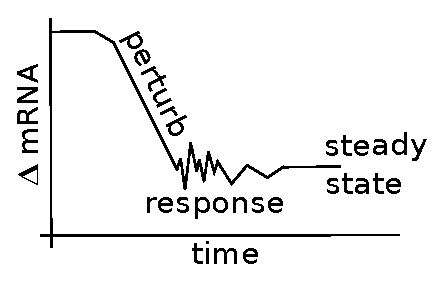
\includegraphics[width=.5\linewidth]{4/pert.eps}
\caption{\textbf{Arrival at steady state after perturbation.} Over time a system will recover from the shock of its initial perturbation to reach some altered, new steady state.
}
\label{fig:SS}
\end{figure}

The assumption of biological systems stability is best framed in view of the alternative hypothesis, that is if systems were unstable, any minor variation, over time, would lead to system collapse \citep{khalil1996adaptive}. A simple way to ensure stability in any dynamic system, and in fact quite a divisive topic in the inference community in particular, is the inclusion of self-regulation in the network. The self interaction plays out indirectly as regulators are transiently expressed to carry out some function, they must then be degraded to reduce cease this response functioning. For example, self-regulation through degradation may be achieved as a secondary effect, wherein buildup of a sought after heat shock response element reaches a critical threshold wherein a cleavage factor creates a byproduct which then binds to the upstream promoter region to shut down heat shock response it partially helped initiate. The cyclic nature of regulatory pathways (\cite{yi2000robust}, see \cref{fig:DNA}), relationship can be seen as inversely proportional, for the quicker this initial factor is expressed, the more of it will surpass this threshold before actively stopping its production and cleavage. Depending on the time delay before byproduct expression and activity is felt, more or less byproduct will be available for cleavage to signal slower or faster overall heat shock response death. This simple indirect feedback mechanism, in concert with other factors, can control quite complex cellular features, such as are described in \cref{sec:pat}. A handful of inference methods disregard this auto-regulatory behavior altogether (ARACNe \citep{montes2014aracne}, CLR\citep{faith2007large}, Genie3\citep{GENIE3}, PLSNet\citep{ham1996partial}). Still others insist on a large portion of measured genes carrying out self-regulation to some degree, ensuring their own expression does not go unchecked, thus destabilizing the system.

As detailed in \textbf{Paper II}, several (penalized) regression based GRN inference methodologies implicitly consider the stability of the system they infer. \textit{Stability selection} uses LASSO under randomized parameterization \citep{tibshirani1996regression} in combination with the irrepresentable condition \citep{zhao2006model}. More reliable GRN inference was demonstrated under a stability criterion by choosing links with subsampled frequencies above an expected upper false positive boundary,  \citep{meinshausen2010stability}.  \textit{Random LASSO} \citep{wang2011random} improves link selection by averaging across bootstrapped distributions of randomly selected subsets of the data, while \textit{TIGRESS} combines stability selection with iterative least angle regression (LARS) estimation \citep{haury2012tigress}.

\subsection{Patterns}
\label{sec:pat}
Life may be presented with any number of stimuli at any given time, and it is only through the mechanism of evolutionary discovery that an adequate response is reached. The cell has many tools to combat an external offense, triggering unique patterns of interaction amongst numerous individual components as an innate response mechanism occurring on a scale of time deemed necessary by evolutionary predictability, \ie what has allowed for survival before. These individual component \textbf{motifs} and their respective responsiveness flow into and out of one another to compose increasingly complex mechanisms of survival. Examples of motifs studied in \coli  and \yeast alike are \textbf{feed-forward loops} (FFL) and \textbf{feedback loops} (FBL).  FFL can amplify the response to an initial stimuli resulting in a quicker response to a potentially deadly threat, while FBL can help to stabilize such response after time has been allowed for its effect to carry out by targeting the very factor initially called for in response to the stimuli to be regulated in the opposite direction initially called for in response \citep{milo2002network} \citep{mangan2003structure}. Others motifs include multi- and single- input module (MIM/SIM), dense overlapping regulons (DOR), and regulator chains \citep{kalir2005coherent} \citep{lee2002transcriptional}. Other methods of robust adaptation in  \coli include bistable systems featuring hysteric behavior where feedback coefficients are greater than one, and oscillatory behavior regulating systems at levels of complexity as high as circadian rhythms \citep{szallasi2006system}.

Motif patterns are identified by comparison to random and are thus agnostic of node makeup, and thus should not be confused with a network module. \textbf{Modules} are composed of select genes \eg to perform distinct functions including transcription and signaling, and are thus seen to be highly conserved across species \citep{alon2007network}. Completely connected subgraphs, known as cliques, appear as motif elements in \yeast at a conservation rate of nearly 50\% among 5 higher eukaryotes, often sharing a common functional class \citep{wuchty2003evolutionary}. This would indicate that some patterns, specifcally those involving all elements in some way regulating all other elements, are so advantageous that in certain circumstances gene function is preserved through huge extents of evolutionary time.

\subsection{Properties}
\label{sec:prop}
\subsubsection{Condition}
\label{sec:cond}
It is important to distinguish data properties from systems (network) properties. Systems generally account for their ability to \emph{handle} noise by estimating the worst case scenario for noise to change the system structure. The distinction is made in network inference of terming this conditioning as \textbf{interampatteness} (IAA, short for INTERactions enabling simultaneous AMPlification and ATTEnuation of different signals), to call attention to it in more general dynamic systems and nonlinear environments \cite{nordling2009interampatteness}. Furthermore, the former is an inherent biological network property while the later also depends on the experimental design matrix.  Thus this interampatteness degree is a measure of the ability of the system to amplify certain signals while attenuating others whose signal is often riddled with systemic noise. This property feeds nicely into another, related property (see \cref{sec:rank}) which is also concerned with multicollinearity, wherein features are functions of one another.

\subsubsection{Rank}
\label{sec:rank}
Rank is another property worth consideration in the context of network inference, specifically in the subcontext of the generation of synthetic data and bootstrapped datasets. As aforementioned, we seek to infer networks where all genes regulate or are regulated, \ie a system which each constituent plays a part. Therefore, if any two or more genes share highly correlated patterns among their readout genes when perturbed, their component system is seen as containing redundant information, \ie the system is \textbf{rank deficient}. It is therefore, firstly advantageous to design datasets composed of genes likely to act and respond independently from one another, as the information content of the dataset is then maximized among the measured genes \citep{subramanian2017next}. Here we further ensure full rank of either matrix type so to guarantee experimental independence and thus prevent inference using less informative datasets. It has been shown that measuring more variables than are experimented upon, and vice versa, is a recipe for lessening the information content of a dataset \citep{Nordling2013}. This simple but computationally non-insignificant, preventative step assures users not remove information from a system.  If any genes correlate too closely (dictated by angle, being the arc cosine of the dot product between the vectors) (\cref{fig:dend}) some fraction of the delinquent genes should be removed from the dataset lest it risk being ill-conditioned or rank deficient.

\begin{figure}[H]
\centering
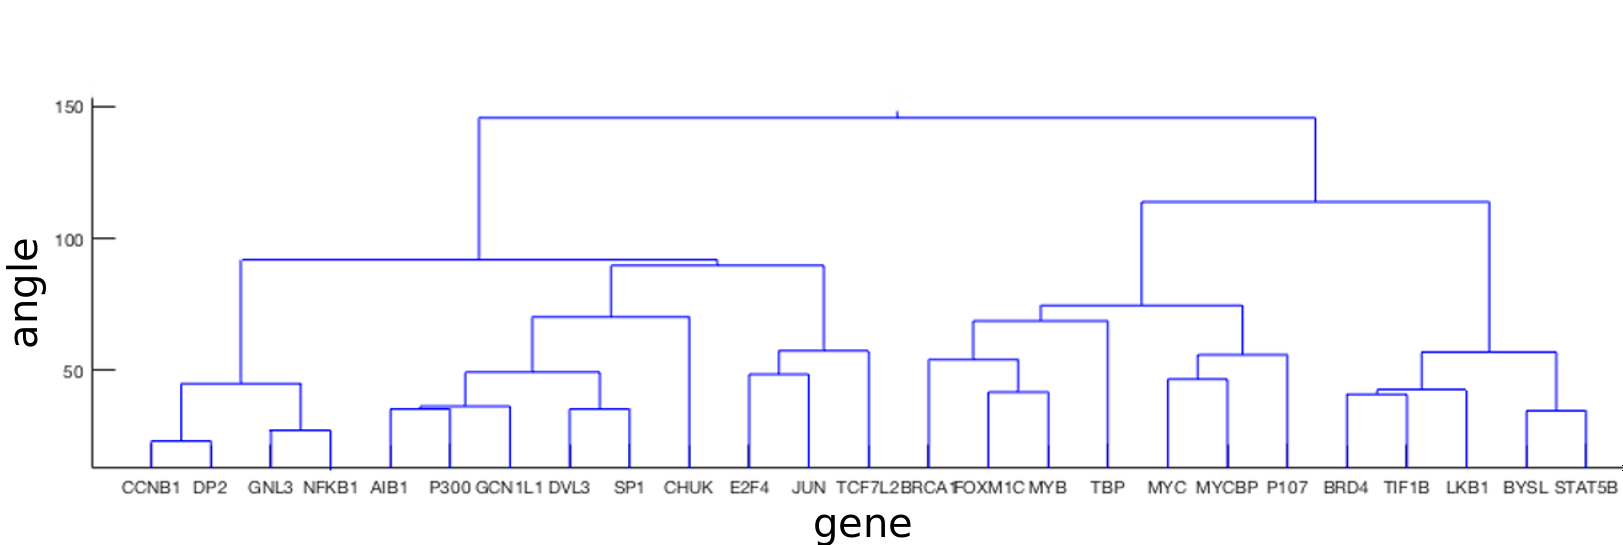
\includegraphics[width=1\linewidth]{4/MYC_Y_weightedDouble_dendrogram.png}
\caption{\textbf{Abbreviated view of MYC double perturbation angle dendrogram}, as an example indicating independence of gene expression via correlation in dataset.}
\label{fig:dend}
\end{figure}

\pagebreak

\subsubsection{Noise}
\label{sec:snr}
As we have seen, systems are often riddled with noise, relying on mechanisms to maintain sufficient conditioning \cref{sec:cond} and rank \cref{sec:rank} to regulate survival; those investigated here are no exception. We aim to \emph{handle} such noise, much the way the natural system does, and its effects on our modeling as it is partially a byproduct of the naturally robust biological system, made worse through the imperfect methods of quantizing a continuous, dynamical system at a single point, not to mention the quantification machinery. Simulating noise is thus equally crucial, and thus we implement a normally distributed model of noise, based on the standard deviation witnessed within measured expression to approximate this inherent noise. Recent findings suggest this may not be optimal, but it allows our models to dynamically represent possible sources of error when inferring networks, which flexibility would not be as forgiving in its absence.

Experimentally, we estimate the \emph{Signal-to-Noise Ratio} (SNR, \cref{eq:SNRl}). of the system assuming normally distributed noise as follows,

\begin{equation}
	\SNR_{\mY\, \normall} \triangleq \frac{\underline{\sigma}(\bY)}{\sqrt{\chi^{-2}(\gamma,NM)\lambda}},
  \label{eq:SNRl}
\end{equation}

where $\underline{\sigma}$ represents the smallest non-zero singular value, $\normall$ the normal distribution with mean $\mu$, variance $\lambda$ and $\chi^{-2}(\gamma,NM)$ is the inverse chi-square distribution with \emph{NM} ($genes \times experiments$) degrees of freedom at significance level $\gamma$ as defined in the supplement to \textbf{Paper I}.

In the case of simulation, wherein a network is initially created, datasets of various data property makeups are created by scaled SNR, a process that defines the E matrix. As such the SNR calculation is more straightforward and exact, where the smallest singular value of Y divided by the largest singular value of E (\cref{eq:SNRt},\cref{fig:SNR}).

\begin{equation}
    \SNR_{\mY\,true} \triangleq \frac{\underline{\sigma}(\bY)}{\overline{\sigma}(\bE)}.
  \label{eq:SNRt}
\end{equation} 

% \begin{wrapfigure}{Hr}{0.5\textwidth}
\begin{figure}[H]
  \begin{center}
    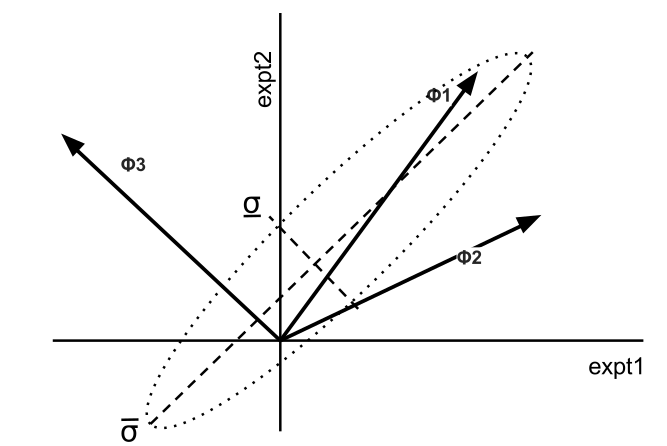
\includegraphics[width=1\linewidth]{4/matrixSNR.png}
%     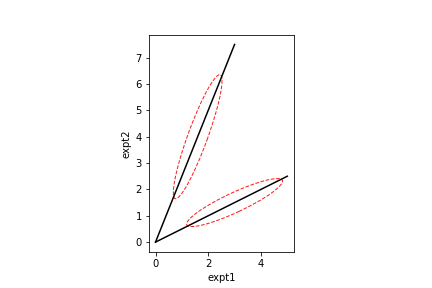
\includegraphics[width=.5\linewidth]{4/SNR.png}
  \end{center}
  \caption{\textbf{Regression lines of two experiments with ellipsoid SVD.} We make the conservative assumption that the minimum eigenvalue across the geneset is a fair proxy to calculate signal-to-noise (SNR) in relation to what is expected under the null $\chi^{-2}$ distribution.}
  \label{fig:SNR}
\end{figure}

\subsubsection{Sparsity}
\label{sec:spar}
The field of network inference aims above all else to determine interactions of consequence, those which affect other system constituents rather than laying idle and isolated. As such, the task must consider to which degree to consider a link is deemed valid, to what degree it initiates a response in its neighbor(s), \ie its link weight. This is done in many methods at once, by a sparsity parameter, $\alpha$, which incrementally returns networks of lesser or greater link weight, as determined by the inference method itself, creating a gradient of networks of increasing \textbf{density} (decreasing sparsity) as weaker link weights are forced into inclusion (\cref{fig:confusion}). Finding the optimal sparsity is an ongoing field of research \citep{tjarnberg2013optimal}. Several different methods were employed throughout this work to determine a single, \emph{best} inferred network, often for comparison between methods or for heuristic reasons of biological relevance (\ie generally containing 3-4 links per node \cite{tjarnberg2013optimal}).The number of nonzero elements is limited using methods which place constraints on total link numbers, \eg the L1 norm in LASSO (\cref{eq:linLASSO}, discussed in depth in \cref{sec:reg}) and a cutoff for ordinary least squares LSCO and total least squares (\cref{eq:LSCO},\cref{eq:TLSCO}, and \cref{sec:regress}). Our R shiny web app ''CancerGRN'' (\cref{fig:GSweb}) which employs several network viewers to display networks at each sparsity level, a few crucial network properties, as well as displaying the overlap support plot for those GRN inferred using \emph{NestBoot} via \textbf{Paper II}.


\begin{figure}
\centering
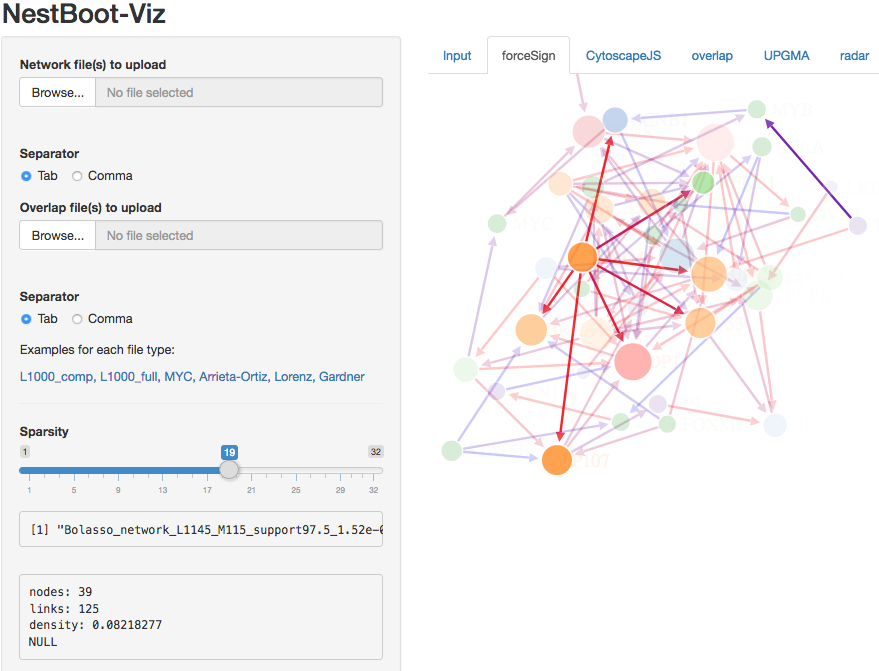
\includegraphics[width=1\linewidth]{4/NestBoot-Viz2.png}
\caption{\textbf{Screenshot of Network Viewer ''Cancer GRN'' Tool.} It offers a network view of variously sparse networks returned from inference, in addition to NestBoot support plots and several general network properties for statistics for comparison. Live at \url{https://dcolin.shinyapps.io/cancerGRN/}}
\label{fig:GSweb}
\end{figure}

\subsection{GRN Modelling Architectures}
\label{sec:models}
As we have discussed, there are many approaches that can be taken to understand relationships among biomolecules. Generally inference methods can be categorized into four model architectures: boolean, bayesian, information theoretic and differential equations \citep{HECKER200986}. An overview of the latter tthree follows the cursory allusion to information theoretic methods in \cref{sec:sysdyn} and the introduction to ODE detailed in \cref{sec:parest}.

% \subsubsection{Probabilistic/Boolean/Petri Nets (PNs)}
% \label{sec:prob}
\subsubsection{Information Theoretic}
\label{sec:info}
The \emph{tree-based} method Genie3 \citep{irrthum2010inferring} uses the equivalent of \emph{supervised} (\textbf{non-parametric}) learning feature selection to determine those genes directly influencing expression patterns of other genes, ranking such features via the tree building process. Thus, it is able to account for \textbf{multifactorial}, \ie unknown perturbation, in the hope of finding genes with expression predictive of target gene expression. As we have seen, this is quite opposing the majority of investigated methods herein, regression methods requiring a perturbation design matrix. The \textbf{ensemble} approach used in Genie3 improves prediction by averaging among bootstrapped trees, each a part of the initial sample space iteratively fragmented from logical demonstrations of single input variable.

% \begin{figure}
% \centering
% 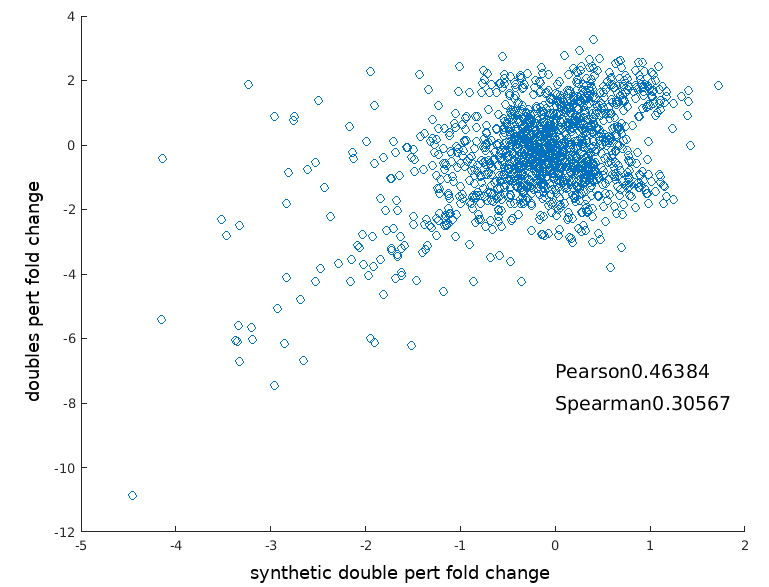
\includegraphics[width=.75\linewidth]{4/doubleVmeanD.png}
% \caption{{Observed multiple perturbations fold change compared to expected.} The correlation of multiple perturbations with their synthetic expected fold changes, \ie double perturbations made from averaging relevant single perturbations. The two are imperfectly related to a degree, ie to .3 and .46 spearman and pearson scores.}
% \label{fig:meandouble}
% \end{figure}


\emph{Mutual information} based inference methods generally define a similarity metric between profile patterns of any two genes, a marginal dependency or \textbf{coexpression}, on a gene-by-gene pair evaluation basis. An obvious distinction arises in that any such method differs from the {\it all-at-once} approach of regression methods \cref{sec:regress} such as LASSO, (Total) Least Squares, \etc. Relevance networks set a threshold above which any regulatory gene pair is identified as a link as a form of clustering \citep{faith2007large}. ARACNe implements an information-theoretic property, the data processing inequality (DPI), to threshold indirect links, seeking to increase true positive recovery while minimizing false positives. Below a certain DPI, the lowest link of three completely linked nodes is removed; otherwise the triangular clique is maintained \citep{montes2014aracne}. CLR, short for Context Likelihood of Relatedness, likewise utilized mutual information (MI) between all genes to estimate likelihoods for each compared to a MI background distribution. This null model is constructed from the MI sets between all possible links, most being that of random background MI due to biological GRN sparsity \citep{faith2007large}. In short, it applies normal distribution statistics to mutual information scores in order to identify network links. (B)C3NET \citep{altay2010inferring},\citep{de2012bagging} corrects for all possible inferred links via a maximization step where they ''bag'' significant links after hypothesis testing.



% \subsubsection{Association: beyond MI \citep{werhli2006comparative}}
% \label{sec:GGM_BN}

% \emph{Relevance networks} consist of association scores composed of mutual information and bolstered with Pearson correlation between nodes, and as such, is not carried out in the context of the system but adheres to the main criticism of MI methods, inspecting nodes element-wise.

Several problems arise reading relational information in this way, least of which is ambiguity in the nature of the cause and effect. Imagine the unique GRN implied by one three node coexpression clique with no manner of discerning among the possible distinguishing features, \eg $A\to B\to C$ versus $ B\to A\to C$ \citep{markowetz2007inferring}.
Graphical Gaussian models (GGM) are examples of full conditional, undirected probabilistic network models estimated from a covariance (\ie concentration or precision) matrix, which \textbf{partial correlation coefficients} are taken as directed, regulatory edges. This partial correlation acts as the strength of the direct, indirect or joint interactions between biomolecules. Whereas correlation networks return degrees of correlation for most genes, drowning out weaker dependent correlation by thresholding for high independent correlation, GGM return more likely interdependent regulations\citep{schafer2004empirical}. However, issues of rank and sparsity arrise when such GGM-based methods scale to larger datasets. In a logical progression toward independence of all orders, \emph{Bayesian networks} (BN) return directed links between given variables, and are thus distinguished as being DAGs representing interaction probabilities between multiple biomolecules. Partial DAGs are also used to collapse unique but equivalent skeletons of the same structure, \ie directionality is disregarded for all links showing bidirectionality between models.


\subsubsection{Perturbation-based Inference}
\label{sec:ODE}
A fundamental element of the inference contained within \textbf{Paper I-IV} lies in their experimental design, namely that response is measured after the system is given time to adequately respond to, \ie reach steady state, an external stimuli, namely a directed knock-down suppression of a gene expression. The technique used to perform the knock-down (KD) is also not immune to introducing error. KD via short hairpin RNA (shRNA) and small interfering RNA (siRNA) are designed to target genes, but given the robust flexibility demonstrated of biological systems to this point, it stands to reason that even primers targeting specific sequence are not entirely unique, and indeed are naturally propagated through the genome. As such, several such primers which identify the target RNA sequence to suppress are either pooled together after reading or introduced as a cocktail, respectively, to mitigate off-target effects. In this way, all genes are systematically targeted with relative affinity, and the expression of readout genes (those not knocked down) are measured. This is a delicate yet imprecise balancing act, where one seeks mitigation of singular effect without irreparably altering the system, rewiring its connections and measuring an altogether different system. 

As is expertly stated in the 2018 Blum \etal publication, "Inferability of a directed link between source and target node requires that the remaining network may not contain the same information that is transmitted between them. A sufficient condition is that all information that the remaining network receives from the source node is destroyed by sufficiently strong perturbations. If the target node is not perturbed, information from the source node may reach the remaining network through the target node" \cite{blum2018experimental}. As such, the synthetic datasets contained with papers presented here \textbf{Papers I-IV} more strictly adhere to this absolute principle. However, real experimental knock downs only achieve this in part, and to varying degrees at that (see Fig. S2 in the \textbf{Paper III} supplement).

Furthermore, unlike correlation or mutual information based methods searching link-by-link to gradually forming a topology, inference using perturbation-based methods is an {\it all-at-once} procedure, \ie LSCO, TLSCO, LASSO (\crefrange{eq:LSCO}{eq:linLASSO}). Such methods here utilize a known experimental design in the form of a experimental design matrix, \ie $\mP$ to better inform the mapping of experimental dataset to the network structure. This design matrix links fold change patterns to interaction pairs in the network. Additionally, it aids in synthetic dataset creation, the network inference process run in reverse, a hugely important feature of the GeneSPIDER toolkit as well as the work contained here. Whereas Genie3 is designed to account for multifactorial unknown or undefined perturbations, here perturbations must be explicitly stated in this design matrix to be taken into account in the inference of an overall GRN topology. 
% Our linear methods are able to account for known perturbation designs orders greater than one as exemplified in part one of our validation study for the perturbation inference study (\cref{fig:meandouble}). 
The \emph{ensemble} learning based ENNET \citep{slawek2013ennet} also relies on experimental design matrix, but to a different effect, considering it when TFs are estimated to target individual genes. Each such subproblem is solved using Gradient Boosting Machine which estimates TF importance or ability to regulate targets, which are evaluated systematically.

\subsubsection{Integrative Methods and Bipartite Graphs}
\label{sec:bipart}

The value and meaningfulness of any given network increases as it more accurately reflects the true dynamic nature of any given biological system. Thus as more platforms are born it is not only advantageous but necessary to integrate this disparate information into a single network, be it GRN or other when considering \eg proteomic data, \etc. In this way, \textbf{Fused regression} \cite{lam2016fused} weighs various levels of biological data with overlapping data points by their quality to integrate several data types to more accurately reverse engineer given regulatory networks. In this way, and in conjunction with the lab's \textbf{Inferelator}\cite{bonneau2006inferelator} inference method, the fused regression package allows the integration of many biological levels of data toward inference of the network encompassing the amassed data, returning a more relevant and biologically meaningful network for its efforts. However, for its strengths, it is reliant upon an initial orthology for how to communicate relationships between and amongst the differing data level elements, ie mapping genes to their respective TFs in the form of expression values, block matrix of transcription factor expression values and regression coefficient values which define the regulatory relationships between TFs and their target genes. Their approach  calls for parameter optimization in addition to using L2 penalization followed by thresholding to return a similar sparsity gradient as L1, while also ranking interactions more accurately.

Similarly, \textbf{PANDA} (Passing Attributes between Networks for Data Assimilation) \cite{glass2013passing} initiates a cooperativity network based on reliance of three levels of biological data -- TF, protein-protein interaction and sequence motif to represent responsibility via outgoing influential links and availability or the incoming ability to be regulated. In this way Glass \etal are able to reconstruct genome-wide, condition-specific regulatory networks by weighing and integrating these data in a manner which cross-checks the \emph{availability} of a target gene to be regulated by a TF against its likely the \emph{responsibility} a TF is measured to have in regulating that gene. Somewhat of a limitation lies in the ability to weigh sources of data relative to their noise level, or any other criterion; however this is easily remedied before incorporation of various data into the final GRN.

\subsection{Methods for Network-Network Comparison}
\label{sec:net_com}
A link-by-link comparison between networks \cref{fig:dend} suffers from the same shortcomings that ultimately limit differential expression analysis (DEA), namely that each piecemeal approach isolates the most highly functioning links or genes, disregarding the state space within which these elements carry out their action. Each analysis is ultimately a study of driving forces defined by fundamental changes in the respective GRNs. Therefore any single gene-gene links on its own cannot suffice when seeking to understand systems dynamics, and instead links between highly differential elements must be preserved and compared, in the form of clique or module comparison. Whats more, these highly interacting and interdependent groups form larger targets as potential biomarkers for therapeutic intervention, wherein knocking out or perturbing in some way one element of a module could more feasibly bring about a positive response than the more strict targeting of single, unrelated gene lists returned from DEA or the link-by-link comparison.
%% above inspired by own thoughts which are reflected in sixth paragraph of ALPACA discussion

% \begin{wrapfigure}{Hr}{0.75\textwidth}
\begin{figure}
\centering
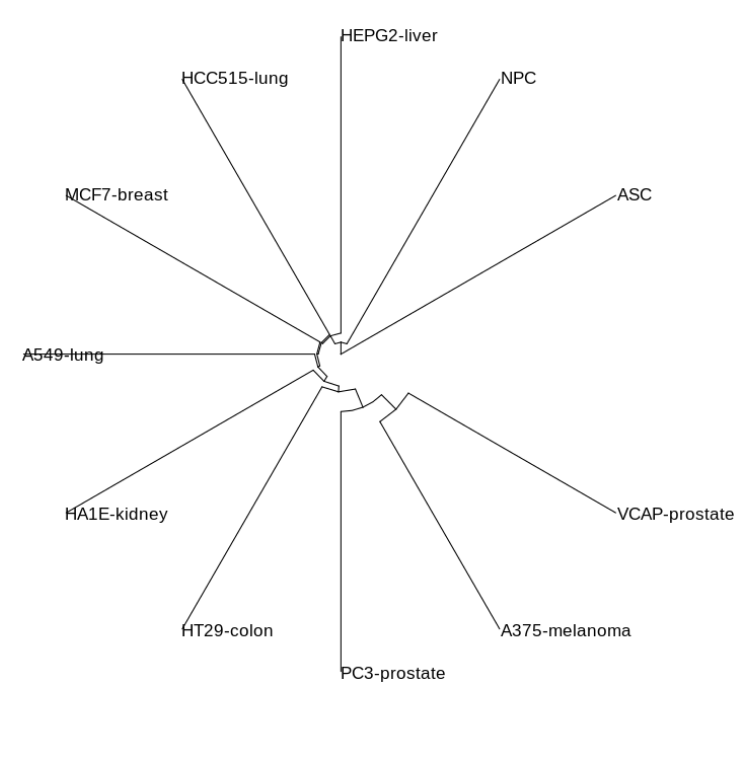
\includegraphics[width=.75\linewidth]{4/better_dendrogram.png}
\caption{\textbf{Link-by-link GRN comparison as dendrogram.} Comparing initial LINCS cell line NestBoot GRN from early investigations in \textbf{Paper IV}. Image taken from expanded capability of the cancerGRN tool (\cref{fig:GSweb})}%. Live at \url{https://dcolin.shinyapps.io/cancerGRN/}}
% \label{fig:dend}\end{wrapfigure}%{Hr}{0.5\textwidth}
\end{figure}

Beyond na{\"i}ve link-by-link comparison, there exist sundry methods for comparing modularity between networks of various levels of sparsity, \eg derived from different time points and obviously between healthy and disease derived cell line. \textbf{CONDOR} (COmplex Network Description Of Regulators) \cite{platig2016bipartite}, seeks to improve regulatory network applicability to medicine by laying out not just gene-gene regulation, exploiting a modified Louvian algorithm to identify groups of upstream SNP regulators responsible for the initial gene regulations. In this way CONDOR can exploit GWAS study data associating many regions of the genome to certain diseases, thereby associating genome abnormalities to the regulatory mechanisms which bring about their phenotypic end, as mentioned in \cref{sec:practical}. Like CONDOR, \textbf{ALPACA}(Altered Partitions Across Community Architecture) \cite{padi2018detecting} utilizes a Lovian variant to detect modularity conservation as well as divergence within networks constraining only on the basis that certain levels of similarity are shared. Another approach at comparing networks inferred from different states is \textbf{MONSTER} (MOdeling Network State Transitions from Expression and Regulatory data) \cite{schlauch2017estimating}, which allows tracking state transition through time or disease progression by weighing elements \emph{directly} and \emph{indirectly} observed. While these methods were designed for specific tasks, they can be repurposed to make other comparisons outside of their TF, SNP, \etc published use cases scenarios. The UpSet \cite{lex2014upset} intersection visualization package carries the prospect of one-to-one network comparisons further, allowing for interactive queries to find combinations of networks from a given set who share given links.

% \subsubsection{Metrics}
% \label{sec:met}
%  -- wRSS, AIC/ BIC
\subsection{Accuracy}
\label{sec:acc}

Much like you hear about the field of statistics, in bioinformatics it similarly stands that whatever you are trying to prove is entirely dependent on the metric you chose to define it. This follows from how interwoven systems biology is with statistically based analytic tools but is nevertheless alarming, that there exists an incredible power to bias, knowingly or unknowingly, results to be more meaningful than they would otherwise seem. My research has often gone out of its way to portray results in a most conservative way possible, sure that as often as something seems certain, there are surely many ways in which the mechanisms we hope to describe are not isolated, \ie system noise amongst signal.

When it came time to score accuracies for inference of networks from synthetic dataset which also contained true gold standard network, we had a few metrics to choose from, all highlighting different ratios of four essential concepts, collectively contained in what is known as a confusion matrix. In this context, \textbf{TP} and \textbf{TN} are links which exist or do not exist in the true gold standard network, respectively, whereas \textbf{FP} and \textbf{FN} are those links inferred incorrectly as existing and not existing, respectively.

\begin{figure}
\centering
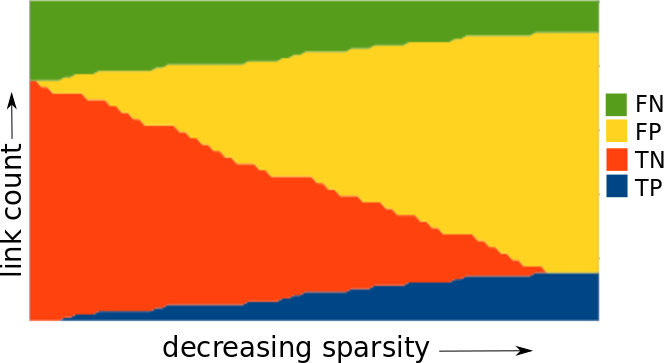
\includegraphics[width=1\linewidth]{4/confusionMatrix_sparsity.png}
\caption{\textbf{Generic confusion matrix in plot form across sparsity levels.} The sparsity decreases left to right. In this example, you see an initial empty network (leftmost) forced to sacrifice any TP link in place of capturing all TN. As links are added (moving right), some FNs are exchanged for TPs or FPs, while other TNs are shifted to FPs as links are forced into the network as it becomes full. Every inference method starts and ends with these network makeups, the empty network a mix of FN and TN, while the full network cannot by definition contain TN. The intervening space is unique per inference method and its parameter setting. Thus finding the most accurate network is a method of balancing the ratio of these links whereby your any metric of accuracy estimation returns an optimal score.}
\label{fig:confusion}
\end{figure}

These individual link scores can be summarized and placed in relation to one another in various ratios. For the purpose of scoring each network individually we chose to report accuracy using Matthews correlation coefficient (MCC) (\cref{eq:MCC}) defined as follows,

\begin{equation}\label{eq:MCC}
MCC=\frac{TP*TN-FP*FN}{\sqrt{(TP+FP)(TP+FN)(TN+FP)(TN+FN)}}.
\end{equation}

This is a somewhat different approach from the inference summary statistics AUROC (\cref{eq:AUROC}) and AUPR (\cref{eq:AUPR}) which rate accuracy across all network sparsities as follow,
%  \begin{subequations}
\begin{equation}\label{eq:TPR}
TPR=\frac{TP}{(TP+FN)},\\ \end{equation}
\begin{equation}\label{eq:FPR}
FPR=\frac{FP}{(TF+TN)},\\ \end{equation}
\begin{equation}\label{eq:AUROC}
AUROC=\sum{TPR*FPR^T}
\end{equation}
% \end{subequations}

%  \begin{subequations}
\begin{equation}\label{eq:PPV} 
PPV=\frac{TP}{(TP+FP)},\end{equation}
\begin{equation}\label{eq:AUPR}
AUPR=\sum{TPR*PPV^T}
\end{equation}
%  \end{subequations}


When one does not have a true gold standard to measure accuracy against, we devised a \textbf{cross validation} method and ultimately use the weighted residual sum of squares (wRSS) (\cref{eqn:wRSS}) in our error balancing procedure when estimating inference accuracy on the novel MYC dataset in \textbf{Paper III}.

\begin{equation}\label{eqn:wRSS}
  \textrm{wRSS}(\zeta) \triangleq \sum_k \frac{||-\bA^{-1}\hat{\bP}_k-\bY_k||^2_2}{cov(\by_k)}+\frac{||\hat{\bP}_k-\bP_k||^2_2}{cov(\bp_k)},
\end{equation}
%   \frac{||\hat{\bP}_k-(\bF_!k\bP^{-1}_{!k}\bP_k)||^2}{cov(\bp_k)}.

where $\hat{\bP}=(\bF_{!k}\bP^{-1}_{!k}\bP_k)$. Keeping with MCC, wRSS is made per network, and thus to evaluate across all sparsities like AUROC or AUPR the cumulative density can be calculated, summing the wRSS per network type. An explicit description of how this is calculated in a cross-validated way is described in the following Author\'s Note, explicitly walking through the BalanceFitError (BFE) algorithm of \textbf{Paper III}.\\

\vspace*{5mm}
\fbox{\begin{minipage}{\linewidth}
\label{note}
\textbf{ Author's Note:}\\
The balancing algorithm in \textbf{Paper III} proceeds by stepwise up and down weighting the limit of the RSS of $\mP$, which constrains $\norm{\mF}$, whos addition to $\mE$ is minimized while solving the equation. Although the limit on $\mE$ is fixed, as the limit on $\mF$ fluctuates, so the smallest solution of $\mE+\mF$ which can solve the equation fluxes. So while $\mE$ starts small when $\mF$ is large (medium weighting), as the limit of $\mF$ becomes smaller (less weight towards RSS $\mP$ limit), $-(\mP-\mF)$ becomes more negative, which means to remain equal to $\mA(\mY-\mE)$, $\mE$ must become bigger, shifting weight from $\mF$ to $\mE$. The trick in inferring genes not present in the cross validation data comes in solving for them as the linear combination of cross validation genes, here  $\hat{\bP}$. In order to alleviate reproducibility bias which arises when the \emph{convex} solution is left otherwise \emph{underdetermined}, this estimated experimental error is balanced as a proxy for the distribution of noise to be expected on the inferred network. \emph{Gradient descent} is implemented using the CVX \emph{convex optimization} \cite{grant2008cvx} MATLAB \cite{MATLAB2017} package to this end. Networks returned are then fit to original data via CLS (\cref{eq:CLS}) to compare against null. 
% \caption{Author's Note}
\end{minipage}}\\


% \begin{figure}
% \centering
% 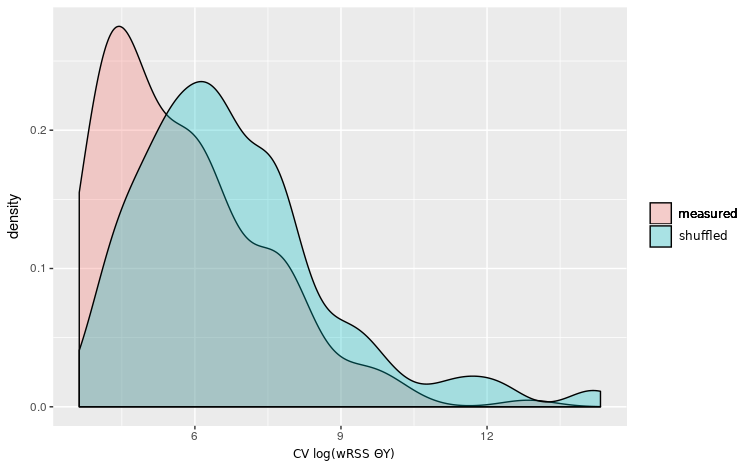
\includegraphics[width=1\linewidth]{4/allDensity_infVrand.png}
% \caption{{\textbf Cumulative Density of wRSS for true Y.} The overall sum of wRSS for all networks of types inferred (red) and random (blue), showing a lower overall error rate for measured networks across all sparsities.}
% \label{fig:CDF}
% \end{figure}




% Frobenius Norm
% Jacobian
% Determinant → schur decomposition
% Chi2inv→ chi2 has cross table structure
% -A-1

% \subsubsection{Ambiguous Benchmarks}
